\documentclass[a4paper]{article}
\usepackage[spanish]{babel}
\usepackage[utf8]{inputenc}
%\usepackage{graphicx}
\usepackage[pdftex]{graphicx}
\usepackage{sidecap}
\usepackage{caption}
\usepackage{subcaption}
\usepackage{booktabs}
\usepackage{float}
\usepackage{color} % para snipets de codigo coloreados
\usepackage{fancybox} % para el sbox de los snipets de codigo
\definecolor{litegrey}{gray}{0.94}
% \newenvironment{sidebar}{%
% \begin{Sbox}\begin{minipage}{.85\textwidth}}%
% {\end{minipage}\end{Sbox}%
% \begin{center}\setlength{\fboxsep}{6pt}%
% \shadowbox{\TheSbox}\end{center}}
% \newenvironment{warning}{%
% \begin{Sbox}\begin{minipage}{.85\textwidth}\sffamily\lite\small\RaggedRight}%
% {\end{minipage}\end{Sbox}%
% \begin{center}\setlength{\fboxsep}{6pt}%
% \colorbox{litegrey}{\TheSbox}\end{center}}

%\newenvironment{codesnippet}{%
%\begin{Sbox}\begin{minipage}{\linewidth-2\fboxsep-2\fboxrule-4pt}\sffamily\small}%
%{\end{minipage}\end{Sbox}%
%\begin{center}%
%\colorbox{litegrey}{\TheSbox}\end{center}}

% \newenvironment{codesnippet}{\VerbatimEnvironment%
%   \noindent
%   %{\columnwidth-\leftmargin-\rightmargin-2\fboxsep-2\fboxrule-4pt}
%   \begin{Sbox}
%   \begin{minipage}{\linewidth-2\fboxsep-2\fboxrule-4pt}
%   \begin{Verbatim}
% }{%
%   \end{Verbatim}
%   \end{minipage}
%   \end{Sbox}%
%   \colorbox{litegrey}{\TheSbox}
% }

\newenvironment{codesnippet}{\VerbatimEnvironment%
  \noindent
  %      {\columnwidth-\leftmargin-\rightmargin-2\fboxsep-2\fboxrule-4pt}
  \begin{Sbox}
  \begin{minipage}{\linewidth}
  \begin{Verbatim}
}{%
  \end{Verbatim}
  \end{minipage}
  \end{Sbox}%
  \colorbox{litegrey}{\TheSbox}
}

\usepackage{fancyhdr}
\pagestyle{fancy}
%\renewcommand{\chaptermark}[1]{\markboth{#1}{}}
\renewcommand{\sectionmark}[1]{\markright{\thesection\ - #1}}
\fancyhf{}
\fancyhead[LO]{AEDA - Take Home Exam}
\fancyfoot[LO]{\small{Iv\'an Arcuschin - 678/13}}
\fancyfoot[RO]{\thepage}
\renewcommand{\headrulewidth}{0.5pt}
\renewcommand{\footrulewidth}{0.5pt}
\setlength{\hoffset}{-0.8in}
\setlength{\textwidth}{16cm}
%\setlength{\hoffset}{-1.1cm}
%\setlength{\textwidth}{16cm}
\setlength{\headsep}{0.5cm}
\setlength{\textheight}{25cm}
\setlength{\voffset}{-0.7in}
\setlength{\headwidth}{\textwidth}
\setlength{\headheight}{13.1pt}
\renewcommand{\baselinestretch}{1.1} % line spacing

\usepackage{caratula}
\usepackage{url}
% \usepackage[usenames,dvipsnames]{xcolor}

% *********************** %
% Otros
\usepackage{natbib}
\usepackage{enumitem}
% \usepackage{multicol}
% *********************** %

\begin{document}
\thispagestyle{empty}
\materia{Seminario sobre Computación, Ciencia y Sociedad en Argentina}
\submateria{Primer Cuatrimestre de 2016}
\titulo{Autonomía nacional y política científica\\ y tecnológica}
\subtitulo{Gustavo F. Bayer}
\integrante{Iv\'an Arcuschin}{678/13}{iarcuschin@gmail.com}
\maketitle
% no footer on the first page
%\thispagestyle{empty}
%\newpage
%\tableofcontents

\newpage
\section*{Repaso de la posición de Gustavo Bayer}
Gustavo Bayer define la \textbf{autonomía general de una nación}  como la capacidad
de un estado nacional para actuar según sus propios intereses. Dicha capacidad
responde a un proceso dinámico en el que no basta con simplemente conquistar la autonomía,
sino que es necesario mantenerla una vez obtenida.

Luego, caracteriza las bases de la autonomía nacional:
\begin{itemize}
    \item Una \textbf{configuración de poder nacional}, que ocurre cuando la acción del estado nacional
        influencia nitidamente las acciones de los otros.
    \item \textbf{Autosuficiencia nacional}, que permite minimizar la capacidad de influencia
        de los otros estados sobre el nuestro.
\end{itemize}

En este escenario, Bayer plantea que el rol de la \textbf{política tecnólogica} es el de:
\begin{itemize}
    \item Suministrar a corto plazo elementos útiles para la ampliación del poder nacional.
        Por ejemplo: explotación y transformación de materias primas. Es decir,
        deberá tender a crear condiciones para la explotación del excedente potencial de los recursos
        naturales. \textbf{Debe lograr adaptar las tecnologías transferidas del exterior a los
        recursos nacionales}.
    \item \textbf{Satisfacer las necesidades sociales}, buscando un aumento de la calidad de vida
        en la población y no solo el aumento de la producción como meta principal.
        Se trata de crear condiciones de oferta para satisfacer necesidades ya existentes,
        y no de introducir tecnología que precisa un mercado consumidor,
        generalmente limitado a las capas de mayor poder adquisitivo.
\end{itemize}

Y el rol de la política cientifica:
\begin{itemize}
    \item Suministrar a largo plazo, los conocimientos necesarios para la sustentación de la autonomía. En particular, \textbf{ampliar y profundizar los conocimientos}, dirigidos por las necesidades del sistema en si, y no caer en el academicismo o la torre de marfil.
        Además se debe buscar una fuerte integración entre las diversas areas del conocimiento adquirido.
    \item Buscar la \textbf{autosuficiencia del sistema cientifico}, buscando la autosustentación, que luego le permitirá actuar como factor de activación de las potencialidades de autosuficiencia nacional a través de la calificación.
\end{itemize}

En resumen, la política tecnológica deberá permitir conquistar la autonomía a corto
plazo, explotando las potencialidades existentes y desarrollandose respetando el siguiente orden:
\begin{itemize}
    \item Recursos nacionales disponibles.
    \item Necesidad de utilización interna.
    \item Posibilidades de su utilización externa.
\end{itemize}

Y luego la política cientifica será la encargada de buscar nuevas potencialidades a ser explotadas, con el fin de mantener la autonomía alcanzada. Además, deberá evitar el clientelismo cientifico, donde el cientifico justifica su investigación diciendo que sirve para el sistema, pero en realidad no.

\vspace{0.5em}

Para finalizar, Bayer hace incapie en que \textbf{debe existir una decisión política de conquista de la autonomía nacional}. No se puede esperar la conquista de la autonomía a partir del crecimiento vegetativo de sus bases de poder y/o autosuficiencia, ya que si una nación que tiene potencialidades de poder no ha logrado su autonomía, es porque existen patrones de dependencia que le impiden despegarse del yugo de los paises desarrollados, junto con barreras sociales o materiales que le impiden alcanzar la autosuficiencia.

En caso de que está decision política no existiese, cualquier crecimiento económico o desarrollo deberá ser encarado con reservas: el crecimiento económico, como benefactor de determinadas capas sociales, concentrador; el crecimiento cientficio, desvinculado de la sociedad como un todo, un crecimiento por el crecimiento (la llamada \textit{torre de marfil}).


\newpage
\section*{Pregunta 1}
\paragraph{Enunciado}
El artículo planea la relación entre la autonomía tecnológica y la autonomía
general de una nación (como oposición a su dependencia).
Comparar la posición de Bayer con la Jorge Sábato y la de Rolando García con relación al mismo tema.

\subsection*{Comparación con la posición de Jorge Sábato}

Abarcaré la posición de Jorge A. Sábato principalmente desde su artículo más conocido con Natalio Botana: \textit{La ciencia y
la tecnología en el desarrollo futuro de América Latina}.

En dicho artículo, los autores presentan un triángulo de relaciones (como el detallado en la Figura \ref{triangulo}) en el cual cada vértice
corresponde a un actor:
\begin{itemize}
    \item Gobierno: el conjunto de roles institucionales que tienen como objetivo formular políticas y movilizar recursos de y hacia los otros vértices a través de los procesos legislativo y administrativo.
    \item Infraestructura científico-tecnológica: el conjunto de sistemas educativos, institutos de investigación, academias de ciencias, etc.
    \item Estructura productiva: el conjunto de sectores productivos que provee los bienes y servicios que demanda una determinada sociedad.
\end{itemize}

\begin{figure}[H]
    \centering
    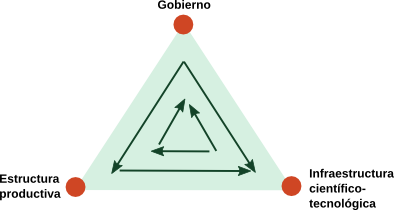
\includegraphics[width=0.6\textwidth]{imagenes/sabato.png}
    \caption{Triángulo de Sábato/Botana}\label{triangulo}
\end{figure}

% Luego, cada vertice tiene responsabilidades y se espera que se relacione con los demás de ciertas maneras.

En el artículo mencionado, Sábato habla de autonomía como la capacidad de decisión propia, y menciona que esta es el resultado de un proceso deliberado de interrelaciones entre los vértices.

Entonces, la postura de Sábato en cuanto a la relación entre autonomía tecnológica y
autonomía nacional se puede analizar desde las responsabilidades que plantea para los distintos vértices, junto con sus relaciones.
% Este proceso se establece a través del flujo de demandas que circulan en sentido vertical (gobierno - los otros dos vertices) y en sentido horizantal.

Sábato distingue tres tipos de relaciones posibles:

\begin{itemize}
    \item \textit{Intrarelaciones}: las que suceden entre los diferentes componentes de un mismo vértice.
    \item \textit{Interrelaciones}: las que suceden entre dos vértices de un mismo triángulo.
    \item \textit{Extrarelaciones}: las que suceden entre dos vértices de triángulos distintos.
\end{itemize}

De las \textbf{intrarelaciones}, basta mencionar que deben estructurarse con vista a garantizar una determinada \textit{capacidad} para generar, incorporar o transformar demandas en un producto final que es la innovación científico-tecnológica. En particular:

% Si hablamos de relaciones internas dentro de cada vertice, \textit{intrarelaciones}, éstas tienen por objetivo transformar a estos centros de convergencia
% en centros capaces de generar, incorporar y transformar demandas en un producto final que es la innovacion cientifico-tecnologica. Es decir:

\begin{enumerate}
    \item El vértice-gobierno requiere la capacidad para realizar una \textit{acción deliberada} en el ámbito de políticas científico-tecnológicas, con el fin de formular un cuerpo de doctrina, de principios y estrategias capaces de fijar metas posibles, cuyo logro depende de una serie de decisiones políticas, de la asignación de recursos y de la programación científico-tecnológica.
    \item El vértice-infraestructura científico-tecnológica requiere la \textit{capacidad creadora}: un científico mediocre producirá ideas mediocres, por más dinero que se les inyecte.
    \item El vértice-estructura productiva requiere \textit{capacidad empresarial}, publica o privada, que se puede definir según las ideas desarrolladas por Schumpeter, como aquella función que ``consiste en reformar o revolucionar el sistema de producción, explotando un invento o, de manera más general, una posibilidad técnica no experimentada para producir una mercancía nueva o una mercancía antigua por un método nuevo, para abrir una nueva fuente de previsión de materias primas o una nueva salida para los productos, para reorganizar una industria, etc''.
\end{enumerate}

El tercer ítem está fuertemente relacionado con las ideas de Bayer de que las políticas tecnológicas deben buscar explotar las potencialidades existentes. Creo además que Sábato concuerda con Bayer en que no sólo hay que lograr innovar en tecnología, sino que ademas ésta debe favorecer el desarrollo social y bienestar general.

\vspace{0.5em}

En cuanto a las \textbf{interrelaciones}, Sábato les asigna una responsabilidad mayúscula: la generación de una capacidad de decisión propia en el campo científico-tecnológico es el \textit{resultado de un proceso deliberado de interrelaciones} entre el vértice-gobierno, el vértice-infraestructura científico-tecnológica y el vértice-estructura productiva.
En mis palabras, Sábato nos dice que la conquista de la autonomía tecnológica depende \textit{fuertemente} de las interrelaciones que logremos construir entre los vértices del triángulo.

Además, Sábato señala que el vértice de la infraestructura científico-tecnológica depende vitalmente de la acción deliberada del gobierno, entendido en un sentido muy amplio, sobre todo en lo que se refiere a asignación de recursos. Sin embargo, el vértice-gobierno juega también el papel de centro impulsor de demandas hacia la infraestructura científico-tecnológica, y es aquí donde reside la dificultad mayor en el modo como se concebirá la formulación de programas una vez tomada la decisión política.

Esta idea concuerda con la posición de Bayer de que \textbf{debe existir una decisión política enmarcada en un proyecto de conquista de la autonomía nacional}. Es decir, que si el gobierno incrementa los recursos de los demás vértices, pero no hace demandas sobre estos, sólo se conseguirá crecimiento aislado, que no contribuirá a la conquista de la autonomía. También es fácil ver que si un gobierno hace demandas sobre los vértices, pero no les provee con los recursos suficientes para funcionar, entonces los resultados obtenidos serán acotados o pobres en su calidad.

\vspace{0.5em}

En cuanto a las \textbf{extrarelaciones}, Sábato afirma: en una sociedad donde funciona el triángulo de relaciones, las aperturas que se realicen hacia el exterior en materia de exportación de ciencia y tecnología original o de adaptación de tecnología importada, producen beneficios reales, ya sea a corto o largo plazo.

Muy distinto es cuando estas aperturas se realizan entre vértices aislados con un triángulo plenamente desarrollado. Este problema es muy característico de las sociedades latinoamericanas, y explica un sin fin de problemas, como por ejemplo el éxodo de talentos. Mientras en nuestras sociedades el científico se encuentra desvinculado y aislado frente al gobierno y a la estructura productiva, en el nuevo lugar de trabajo, al cual lo conduce su exilio cultural, está automáticamente amparado por instituciones o centros de investigación que, a su vez, se encuentran insertos en el sistema de relaciones planteado.

Creo que estas ideas ponen todavía más de manifiesto que Sábato concuerda con Bayer, en la necesidad de un proyecto claro a nivel nacional que busque la autonomía, ya que además comprende que la falta de este trae problemas graves que aumentan la dependencia.

\vspace{0.5em}

Habiendo dicho esto, Sábato afirma que en América Latina no existe un sistema de relaciones como el mencionado, ni tampoco hay conciencia acerca de la necesidad impostergable de establecerlo, por lo que hay una doble exigencia para las naciones en vías de desarrollo que busquen alcanzar su autonomía:
\begin{itemize}
    \item Crear una conciencia global para que nuestras sociedades asuman este problema en sus dimensiones reales.
    \item Actuar eficazmente sobre aquellos sectores en los cuales se podrían optimizar los recursos escasos en función del sistema de relaciones perseguido.
\end{itemize}

Además, Sábato reafirma: corresponde al sector gubernamental formular una política tendiente a \textit{acoplar} la infraestructura científico-tecnológica al proceso de producción, ya sea creando los centros que así lo permitan o relacionando los centros ya existentes.

\vspace{0.5em}

Por último, quisiera dar un ejemplo concreto que presenta Sábato en su artículo \textit{Empresas y fábricas de tecnología}, de la creación en 1971 de una empresa Argentina estatal que responde a necesidades de desarrollo existentes en ese momento, la \textit{Empresa Nacional de Investigación y Desarrollo Eléctrico S.A.} (\texttt{ENIDE}). Su objetivo fundamental estaba definido en su estatuto como ``Producir, distribuir, comprar, vender, exportar, importar e intercambiar conocimiento técnico-científico en el campo de la energía eléctrica y sus aplicaciones'', y su creación obedecía a diversas circunstancias:

\begin{itemize}
    \item La existencia de un mercado importante y en rápido crecimiento.
    \item En el campo de la energía eléctrica, la Argentina era neto importador de tecnología.
    \item Existía capacidad científico-tecnológica apta para la producción de tecnología eléctrica. La demanda interna era, sin embargo, muy escasa y de poca significación cualitativa.
    \item Por tratarse de un tipo de actividad que tenía poca tradición en el país, sobre cuya necesidad no existía aún conciencia clara y que requería capital de riesgo, sólo el Estado estaba en condiciones de ponerla en marcha.
\end{itemize}

% Notas Sábato:
% - no al colonialismo mental
% - pensar el desarrollo tecnologico como motor del desarrollo social y economico del país.
% - solo mediante ese manejo autonomo tecnologico podra una nacion comenzar a marchar
%     en la dirección que eventualmente le permitira disponer en cada caso de la tecnologia más ajustada
%     a sus propios objetivos, más respestuosa de su acervo cultural, más conveniente para sus propias
%     necesidades y más adecuadas a sus dotaciones de recursos y factores.
%
% - tecnologia nacional: manejar la tencologia como mas le convenga al país,
% - ¿Qué desarrollar y que comprar ? A veces conviene desarrollar primero, para luego importar en mejores condiciones.
% - La relacion entre politica tecnologica y economica, es determinante.
% - En particular, el uso del poder de compra del estado es el instrumento más importante
%
% - se va a alcanzar autonomia tecnologica: no como autonomia que reniega de la participacion de tecnologica extranjera,
%     sino como capacidad tecnologica autonoma, de generacion de tecnologia y de incorporacion de tecnologia estranjera a modo de configuracion de paquetes.
%     Lo contrario sería la desagregacion de paquetes tecnologicos, es decir: una participacion de componentes nacionales.
%
% - dependencia tecnologica: incorporación sumisa de las tecnologías disponibles por razones de disponibilidades y precios en el mercado.
% - autonomia: capacidad de desarrollo local: construir el triángulo, interrelacinando los tres vertices. Solo puede pasar si el estado tiene
%     una participacion clave en la estructura productiva.
% - presidente de SERBA: Empieza identificando cuales son los productos en los cuales puede haber desarrollo
%     tecnologico local y en los cuales podíamos prescindir de componentes importados.
% - Industrialización sustitutiva de importaciones.
% - Regimenes de promocion del desarrollo industrial, bastante protectivos: proteger a la industria naciente.
% - De vuelta: el compre nacional es un factor clave para la autonomia tecnologica, muestra una preferencia en cuanto proveedores externos.
% - Regulación de transferencia de tecnología extranjera
%
% -Por tanto, la desagregación tecnológica es también un instrumento de política industrial que busca maximizar
% la participación propia en la ejecución de proyectos de inversión por medio del incremento del componente tecnológico
%  nacional en la producción de un bien o de un servicio. Para eso es preciso investigar, en detalle, los agregados humanos,
%   económicos y técnicos de cada uno de los proyectos de inversión.

% http://www.fundacionsadosky.org.ar/seminario-ciencia-y-tecnologia-en-el-pensamiento-de-jorge-sabato-oscar-varsavsky-y-amilcar-herrera/


\subsection*{Comparación con la posición de Rolando García}

Debido a la dificultad de encontrar textos específicos de Rolando García que hablen de políticas tecnológicas, trataré de abarcar su posición en el tema principalmente desde la charla que dio en el 2006 en la FCEyN, UBA.

En dicha charla, García menciona que:

\begin{itemize}
    \item ``Todo proceso profundo de transformación, en cualquier dominio, comienza con la apertura de nuevas vías de acción''.
    \item ``Las acciones emprendidas sólo tienen sentido si se comprende cuáles eran sus objetivos''.
    \item ``En el contexto particular de las universidades se discute mucho más sobre problemáticas puntuales que sobre el proyecto institucional en el que deberían de estar inscritas. Y es necesario subrayar que existe una gran diferencia entre un proyecto institucional y un programa de medidas propuestas o adoptadas en la coyuntura''.
\end{itemize}

Estas ideas muestran que García, al igual que Bayer, entiende que la conquista de la autonomía de los países en vías de desarrollo no se puede lograr de manera vegetativa, sin tomar acciones concretas al respecto, sino que es necesario buscar nuevas alternativas que permitan romper el ciclo de dependencia (lo que Bayer llama, explotar las potencialidades existentes).

Además, ambos muestran en su pensamiento que no basta que ciertos actores particulares del sistema tomen algunas acciones concretas, sino que hacen falta políticas de estado que se enmarquen en un proyecto de conquista (y luego mantenimiento) de la autonomía.

Con respecto a la autonomía universitaria, García dice:

\begin{itemize}
    \item ``Tener claro en qué consistía la autonomía universitaria y por qué era indispensable defenderla nos permitió negociar con diversas instituciones, incluso extranjeras, para obtener subsidios sin quedar subordinados a las decisiones que muchos intentaron imponer junto con los financiamientos''.
    \item ``Pero la autonomía no significaba, para nosotros, el aislamiento ante los problemas del país y del mundo. Casualmente, revisando en estos días viejos papeles, encontré un documento que vale la pena citar porque tiene que ver, precisamente, con las implicaciones políticas de nuestra posición. Mientras yo mantenía relación con la Fundación Ford y con otras organizaciones norteamericanas, en el año 1965 tuvo lugar la invasión a Santo Domingo. En la Facultad de Ciencias Exactas y Naturales, expresamos nuestra condena con actos públicos''.
    % \item ``Cuando nos propusimos reconstruir la Universidad, en los años 50, enfrentamos una situación comparable en cierta medida. No era suficiente con modificar los planes de estudio, construir nuevos edificios y sustituir el personal docente y administrativo. Era necesario replantear La estructura de la institución, sus objetivos y su funcionamiento, para lo cual se requería mantener a ultranza la autonomía de la gestión. A partir de allí, \textbf{construir lo posible} significó encontrar los medios necesarios para poner en práctica la profunda reforma que nos planteamos como meta''
\end{itemize}

Lo que muestra que García comparte con Bayer la posición de que \textit{la política tecnológica deberá buscar satisfacer las necesidades sociales, buscando un aumento de la calidad en la vida de la población y no sólo el aumento de la producción como meta principal}.

% http://www.pagina12.com.ar/diario/universidad/10-209827-2012-12-14.html
% Siempre entendió que las universidades y los centros de investigación debían estar al servicio de las necesidades populares y que, por lo mismo, la enseñanza y el aprendizaje debían apuntar al rigor y a la excelencia. Todo un jesuita este querido maestro y amigo.

% Charla 2006

% \item ``El haber conseguido Los subsidios de la Fundación Ford, insisto, para la compra de material científico y para otorgar becas externas, despertó ataques en todos los frentes. Por una parte, la derecha se preguntaba cómo era posible que fundaciones norteamericanas apoyaran a una facultad dominada por los izquierdistas y que privilegiara a Las ciencias duras por encima de Las humanidades. (Cabe recordar que la primera gestión que realicé personalmente en Washington con la Fundación, fue para conseguir fondos para La creación del Departamento de Sociología de la Facultad de Filosofía y Letras]. Por otra parte, la obtención de subsidios también despertó ataques por parte de la izquierda, que temía la penetración en el mundo universitario del imperialismo norteamericano a través de Los mismos.''
% \item ``Es necesario aclarar que los subsidios de la Fundación Ford fueron necesarios para el equipamiento de La Unrversidad y para otorgar becas al exterior, no para la construcción de la Ciudad Universitaria, que fue enteramente financiada por el Estado gracias a una partida especial gestionada directamente por Risieri Frondizi, rector de la UBA y hermano del Presidente de la Nación, Arturo Frondizi.''



\newpage
\section*{Pregunta 2}
\paragraph{Enunciado}
 Comparar la posición de Bayer con el planteo general del desarrollismo. ¿En qué se parecen y en qué se diferencian?

 \subsection*{Comparación con la posición del desarrollismo}

 El planteo general del desarrollismo es :
% Youtube: Prebisch y los terminos de intercambio https://www.youtube.com/watch?v=sqUQQX1dTx8
 \begin{itemize}
     \item Los terminos de intercambio en el comercio internacional, con un esquema centro industrial-periferia agrícola, tienden a caer a lo largo del tiempo,  y amplian la brecha entre paises desarrollados y subdesarrollados. Esto es lo que se conoce como la Tesis Prebisch-Singer.
     \item Los paises subdesarrollados deberían combatir este hecho mediante Estados activos, con políticas económicas que impulsen la industrialización, para romper así la asimetria que genera el sistema capitalista dentro de los intercambios internacionales, y alcanzar la autonomía.
    %  \item En vez de que los trabajadores o los empresarios ganen más por ser más eficientes, los precios de los productos bajan, lo que beneficia a los países más ricos.
    \item La amplitud de los ciclos economicos en los países de la periferia es mayor que en los países del centro: cuando hay bonanza economica los precios de las materias primas aumentan porque aumenta la demanda, pero cuando hay contracciones estos caen aún más porque no hay mecanismos institucionales que frenen esa caida.
 \end{itemize}

 Entonces los países en vías de desarrollo deben:

 \begin{itemize}
     \item Buscar la diversificación productiva e integración regional:  superar la limitada diversificación productiva y la heterogeneidad estructural.
     \item Buscar el desarrollo con igualdad: promover un desarrollo con equidad, cimentado en los cambios en la estructura productiva.
     \item Buscar una nueva inserción en el orden mundial: tranformar las formas de inserción de América Latina en el orden mundial
 \end{itemize}

 Las similitudes con la posición de Bayer son:

 \begin{itemize}
     \item Un fuerte enfasis en la existencia de patrones de dependencia que mantienen a las naciones en vías de desarrollo en tal estado.
     \item Además, que hace falta un proyecto de Estado con políticas claras de conquista de la autonomía.
 \end{itemize}

 Y las diferencias:

 \begin{itemize}
     \item El desarrollismo clasico (Prebisch)
 \end{itemize}


\newpage
\bibliographystyle{plain}
\section{Referencias}
\begingroup
\renewcommand{\section}[2]{}
\bibliography{informe}
\endgroup

%\newpage
%\appendix
%\input{apendiceC}

\end{document}
